\section{Тестирование программного продукта}

Разработав отдельные компоненты продукта, необходимо протестировать ее работоспособность на тестовом изображении.

\subsection{Демонстрация программного продукта}
Для создания $\textit{Graphical User Interface (GUI)}$ использовался язык $Python$ и библиотека $tkinter$ \cite{tkinter}, а также $matplotlib$ \cite{matplot}.

При первом входе в приложение будет произведена авторизация путем протокола $\textit{OAuth 2.0}$. На рисунке ~\ref{auth_window} показано окно авторизации через облачное хранилище (в данном случае $Google$)

\begin{figure}
    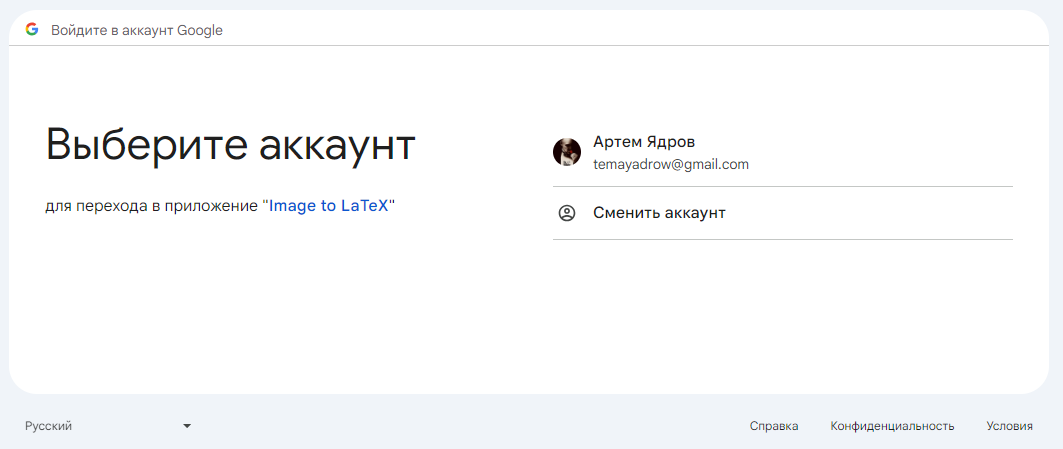
\includegraphics[scale=0.5]{img/app/oauth_1.png}
    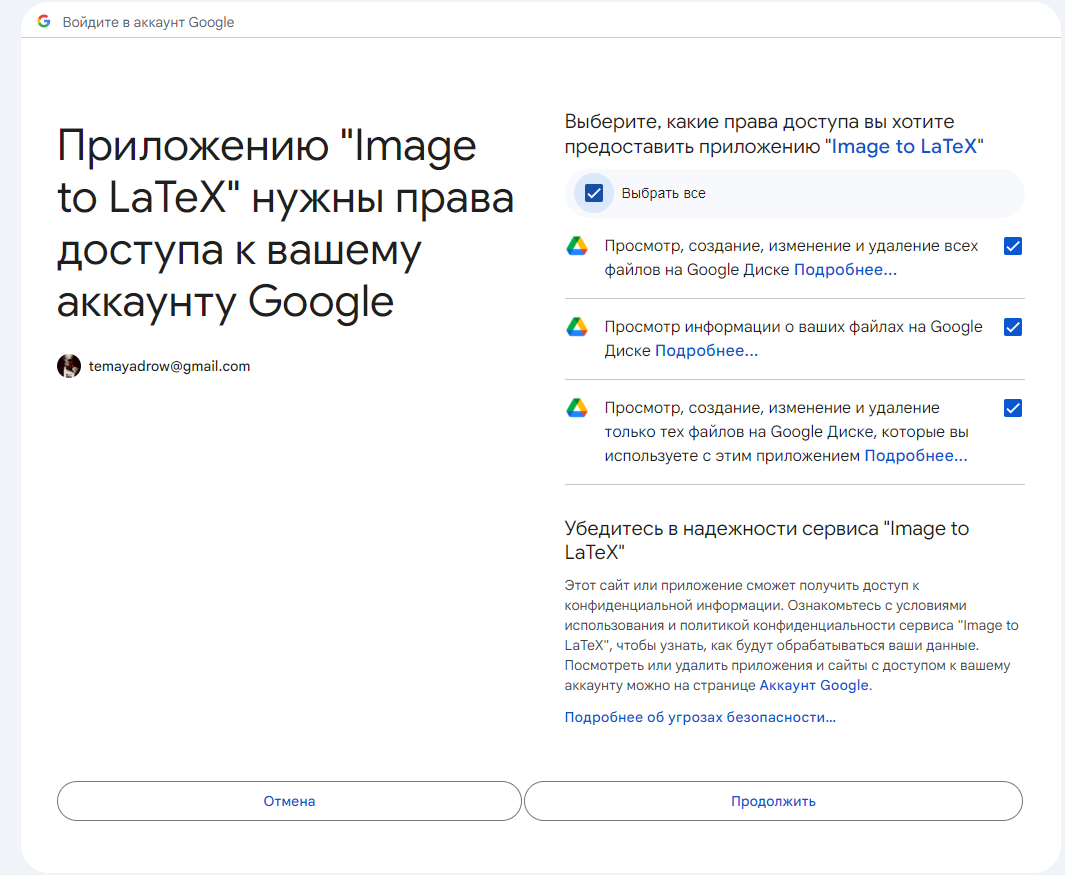
\includegraphics[scale=0.3]{img/app/oauth_2.png}
    \caption{Окно авторизации через облачное хранилище}
    \label{auth_window}
\end{figure}

После выбора изображения, согласно схеме, представленной на рисунке ~\ref{neuro_model}, начинается процесс коррекции перспективы. В случае неудачного изображения может понадобиться коррекция пользователя. В таком случае появляется окно, представленное на рисунке ~\ref{perspective_correction_window}

\begin{figure}
    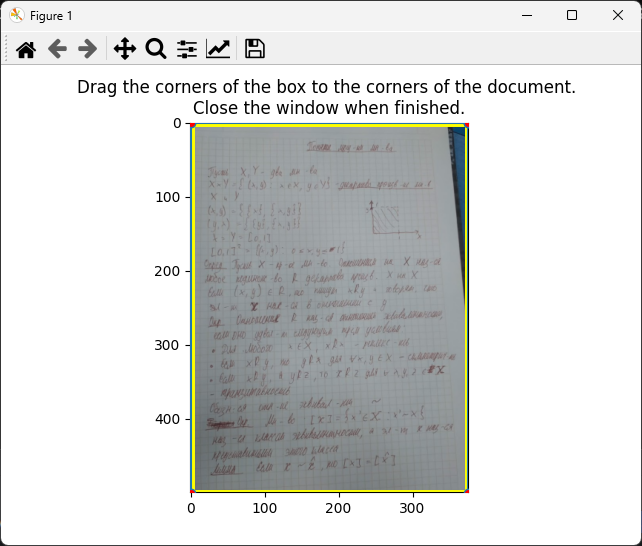
\includegraphics[]{img/app/perspective_correction_window.png}
    \caption{Окно пользовательского ввода для коррекции перспективы}
    \label{perspective_correction_window}
\end{figure}


Изображение с коррекцией перспектктивы выводится на экран пользователя, а также отправляется на сервер, где происходит выделение формул. На клиентской машине в это время производится сегментация на абзацы и дальнейшая ее корректировка, как показано на рисунке